% =====================================================================
% Fig. 1 - FEATHer overall architecture (IoT-J revision, v2).
% Each module box now contains an actual visual sketch of what it does,
% not just text:
%   [1] Multiscale     -> 4 stacked mini-waveforms (point/high/mid/low)
%   [2] Shared DTK     -> sliding kernel over multi-channel strip
%   [3] Freq Gating    -> softmax bar chart over 4 branches
%   [4] SPK            -> period-aligned grid reshape
% Endcaps: input/output mini time series.
% Side input: FFT magnitude spectrum (above [3]).
%
% Standalone compile:  pdflatex fig1_overall.tex
% =====================================================================
\documentclass[tikz, border=8pt]{standalone}

\usepackage{amsmath, amssymb}
\usepackage{tikz}
\usetikzlibrary{
    arrows.meta,
    positioning,
    calc,
    decorations.pathreplacing,
    patterns
}

% branch color palette (kept consistent across Fig. 2-5)
\definecolor{pointC}{HTML}{6B7280}   % gray   (point, k=1)
\definecolor{highC}{HTML}{DC2626}    % red    (high, k=3)
\definecolor{midC}{HTML}{F59E0B}     % amber  (mid, k=5)
\definecolor{lowC}{HTML}{2563EB}     % blue   (low, pooled)

\begin{document}

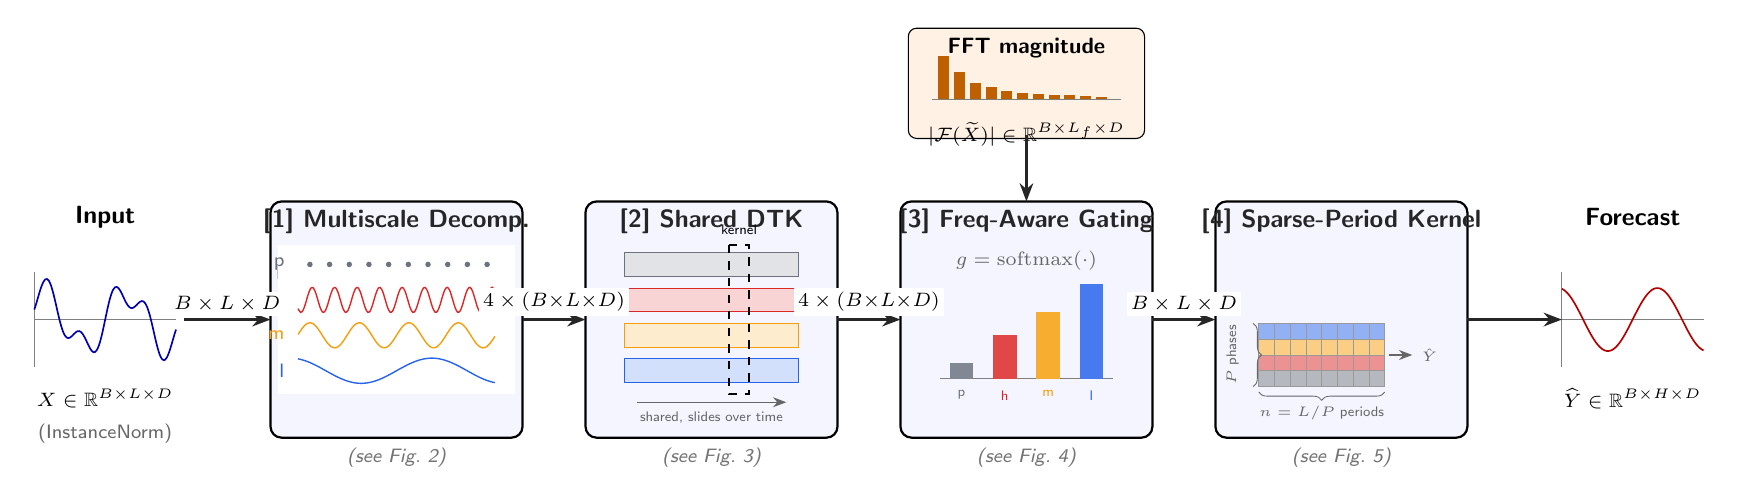
\begin{tikzpicture}[
    font=\sffamily\small,
    >=Stealth,
    mod/.style={
        draw, thick,
        rounded corners=4pt,
        fill=blue!4,
        minimum width=3.2cm,
        minimum height=3.0cm
    },
    side/.style={
        draw, thin,
        rounded corners=3pt,
        fill=orange!10,
        minimum width=3.0cm,
        minimum height=1.4cm
    },
    tag/.style={
        font=\sffamily\scriptsize,
        fill=white,
        inner sep=1.5pt
    },
    ref/.style={
        font=\sffamily\scriptsize\itshape,
        text=black!55
    },
    modlabel/.style={
        font=\sffamily\bfseries\small,
        text=black!85
    },
    flow/.style={->, thick, draw=black!85},
    axis/.style={draw=black!50, line width=0.3pt}
]

% =====================================================================
% Geometry: x positions for each module column.
% Module boxes are 3.2cm wide; centers at x = 0, 4, 8, 12.
% =====================================================================

% ---------------- Input endcap (mini time series) ----------------
\begin{scope}[shift={(-3.7, 0)}]
    \node[font=\sffamily\bfseries\small] at (0, 1.3) {Input};
    % small time-series sketch
    \draw[axis] (-0.9, 0) -- (0.9, 0);
    \draw[axis] (-0.9, -0.6) -- (-0.9, 0.6);
    \draw[blue!70!black, line width=0.6pt, smooth, samples=80, domain=-0.9:0.9]
        plot (\x, {0.35*sin(6*\x r) + 0.18*sin(15*\x r)});
    \node[font=\sffamily\scriptsize] at (0, -1.0)
        {$X \in \mathbb{R}^{B \times L \times D}$};
    \node[font=\sffamily\scriptsize, text=black!60] at (0, -1.45)
        {(InstanceNorm)};
\end{scope}

% =====================================================================
% [1] Multiscale Decomposition: 4 stacked mini-waveforms
% =====================================================================
\node[mod] (M1) at (0, 0) {};
\node[modlabel] at (0, 1.25) {[1] Multiscale Decomp.};

\begin{scope}[shift={(0, 0)}]
    % four horizontal lanes for point / high / mid / low
    % lane y-centers: 0.6, 0.2, -0.2, -0.6
    % point: dots
    \foreach \xi in {-1.1, -0.85, -0.6, -0.35, -0.1, 0.15, 0.4, 0.65, 0.9, 1.15} {
        \fill[pointC] (\xi, 0.6) circle (0.04);
    }
    \node[font=\sffamily\scriptsize, text=pointC] at (-1.45, 0.6) {P};
    % high freq: fast oscillation
    \draw[highC, line width=0.55pt, smooth, samples=70, domain=-1.2:1.2]
        plot (\x, {0.6 + 0.12*sin(20*\x r)});
    % wait — this overlaps with point lane. fix below.
\end{scope}

% redo lanes with cleaner spacing
\begin{scope}[shift={(0, 0)}]
    \fill[white] (-1.5, -0.95) rectangle (1.5, 0.95);  % wipe
    \def\lW{1.25}   % half-lane width
    \def\lH{0.16}   % lane sketch amplitude
    % point lane y=0.7
    \node[font=\sffamily\scriptsize, text=pointC, anchor=east] at (-\lW - 0.05, 0.7) {p};
    \foreach \xi in {-1.1, -0.85, -0.6, -0.35, -0.1, 0.15, 0.4, 0.65, 0.9, 1.15} {
        \fill[pointC] (\xi, 0.7) circle (0.035);
    }
    % high lane y=0.25
    \node[font=\sffamily\scriptsize, text=highC, anchor=east] at (-\lW - 0.05, 0.25) {h};
    \draw[highC, line width=0.5pt, smooth, samples=80, domain=-\lW:\lW]
        plot (\x, {0.25 + \lH*sin(22*\x r)});
    % mid lane y=-0.20
    \node[font=\sffamily\scriptsize, text=midC, anchor=east] at (-\lW - 0.05, -0.20) {m};
    \draw[midC, line width=0.5pt, smooth, samples=80, domain=-\lW:\lW]
        plot (\x, {-0.20 + \lH*sin(10*\x r)});
    % low lane y=-0.65
    \node[font=\sffamily\scriptsize, text=lowC, anchor=east] at (-\lW - 0.05, -0.65) {l};
    \draw[lowC, line width=0.5pt, smooth, samples=80, domain=-\lW:\lW]
        plot (\x, {-0.65 + \lH*sin(3.5*\x r)});
\end{scope}
\node[ref] at (0, -1.75) {(see Fig.~2)};

% =====================================================================
% [2] Shared DTK: depthwise kernel sliding over multi-channel strip
% =====================================================================
\node[mod] (M2) at (4, 0) {};
\node[modlabel] at (4, 1.25) {[2] Shared DTK};

\begin{scope}[shift={(4, 0)}]
    % 4 stacked channel strips (one per branch, same colors)
    \def\sH{0.3}                          % strip vertical thickness
    \def\sLleft{-1.1}                     % strip x range
    \def\sLright{1.1}
    % strip y centers
    \foreach \cy/\cc in {0.7/pointC, 0.25/highC, -0.20/midC, -0.65/lowC} {
        \fill[\cc!20] (\sLleft, \cy-\sH/2) rectangle (\sLright, \cy+\sH/2);
        \draw[\cc, line width=0.4pt] (\sLleft, \cy-\sH/2) rectangle (\sLright, \cy+\sH/2);
    }
    % shared kernel: same vertical bar across all 4 lanes
    \def\kX{0.35}
    \draw[black, line width=0.7pt, dashed]
        (\kX-0.13, 0.95) rectangle (\kX+0.13, -0.95);
    \node[font=\sffamily\tiny, anchor=south] at (\kX, 0.95) {kernel};
    % sliding arrow under
    \draw[->, thin, draw=black!60]
        (\sLleft + 0.15, -1.05) -- (\sLright - 0.15, -1.05);
    \node[font=\sffamily\tiny, text=black!60, anchor=north] at (0, -1.05) {shared, slides over time};
\end{scope}
\node[ref] at (4, -1.75) {(see Fig.~3)};

% =====================================================================
% [3] Frequency-Aware Gating: softmax bar chart over 4 branches
% =====================================================================
\node[mod] (M3) at (8, 0) {};
\node[modlabel] at (8, 1.25) {[3] Freq-Aware Gating};

\begin{scope}[shift={(8, 0)}]
    % baseline
    \draw[axis] (-1.1, -0.75) -- (1.1, -0.75);
    % 4 bars (softmax weights) — heights illustrative
    % position centers at x = -0.825, -0.275, 0.275, 0.825
    \def\bW{0.30}
    % heights: low=0.45 (dominates), mid=0.30, high=0.25, point=0.15
    \fill[pointC!85] (-0.825-\bW/2, -0.75) rectangle (-0.825+\bW/2, -0.75+0.20);
    \fill[highC!85] (-0.275-\bW/2, -0.75) rectangle (-0.275+\bW/2, -0.75+0.55);
    \fill[midC!85]  ( 0.275-\bW/2, -0.75) rectangle ( 0.275+\bW/2, -0.75+0.85);
    \fill[lowC!85]  ( 0.825-\bW/2, -0.75) rectangle ( 0.825+\bW/2, -0.75+1.20);
    % bar labels
    \node[font=\sffamily\tiny, text=pointC, anchor=north] at (-0.825, -0.78) {p};
    \node[font=\sffamily\tiny, text=highC, anchor=north]  at (-0.275, -0.78) {h};
    \node[font=\sffamily\tiny, text=midC, anchor=north]   at ( 0.275, -0.78) {m};
    \node[font=\sffamily\tiny, text=lowC, anchor=north]   at ( 0.825, -0.78) {l};
    % softmax label
    \node[font=\sffamily\scriptsize\itshape, text=black!60, anchor=south]
        at (0, 0.5) {$g = \mathrm{softmax}(\cdot)$};
\end{scope}
\node[ref] at (8, -1.75) {(see Fig.~4)};

% =====================================================================
% [4] SPK: period-aligned grid reshape (P=4, n_periods=3)
% =====================================================================
\node[mod] (M4) at (12, 0) {};
\node[modlabel] at (12, 1.25) {[4] Sparse-Period Kernel};

\begin{scope}[shift={(12, 0)}]
    \def\cw{0.20}   % cell width
    \def\ch{0.20}   % cell height
    \def\gx{-1.05}  % grid origin x
    \def\gy{-0.85}  % grid origin y
    \def\rows{4}    % period P
    \def\cols{8}    % n_periods (input length / P)
    % draw cells, color-cycling by row to show phases
    \foreach \r in {0,1,2,3} {
        \pgfmathsetmacro{\rowy}{\gy + \r*\ch}
        \foreach \c in {0,...,7} {
            \pgfmathsetmacro{\cellx}{\gx + \c*\cw}
            \ifnum\r=0 \def\cellcolor{pointC!50} \fi
            \ifnum\r=1 \def\cellcolor{highC!50}  \fi
            \ifnum\r=2 \def\cellcolor{midC!50}   \fi
            \ifnum\r=3 \def\cellcolor{lowC!50}   \fi
            \fill[\cellcolor] (\cellx, \rowy) rectangle (\cellx + \cw, \rowy + \ch);
            \draw[black!40, line width=0.2pt] (\cellx, \rowy) rectangle (\cellx + \cw, \rowy + \ch);
        }
    }
    % brace under grid: "n periods"
    \draw[decorate, decoration={brace, mirror, amplitude=3pt}, draw=black!60, line width=0.3pt]
        (\gx, \gy - 0.07) -- (\gx + \cols*\cw, \gy - 0.07);
    \node[font=\sffamily\tiny, text=black!60, anchor=north] at (\gx + \cols*\cw/2, \gy - 0.13) {$n = L/P$ periods};
    % brace left of grid: "P phases"
    \draw[decorate, decoration={brace, amplitude=3pt}, draw=black!60, line width=0.3pt]
        (\gx - 0.07, \gy + \rows*\ch) -- (\gx - 0.07, \gy);
    \node[font=\sffamily\tiny, text=black!60, rotate=90, anchor=south] at (\gx - 0.13, \gy + \rows*\ch/2) {$P$ phases};
    % horizon brace right (forecast extends)
    \draw[->, thin, draw=black!60]
        (\gx + \cols*\cw + 0.05, \gy + \rows*\ch/2)
        -- (\gx + \cols*\cw + 0.35, \gy + \rows*\ch/2);
    \node[font=\sffamily\tiny, text=black!60, anchor=west]
        at (\gx + \cols*\cw + 0.35, \gy + \rows*\ch/2) {$\hat Y$};
\end{scope}
\node[ref] at (12, -1.75) {(see Fig.~5)};

% =====================================================================
% Output endcap (mini forecast time series)
% =====================================================================
\begin{scope}[shift={(15.7, 0)}]
    \node[font=\sffamily\bfseries\small] at (0, 1.3) {Forecast};
    \draw[axis] (-0.9, 0) -- (0.9, 0);
    \draw[axis] (-0.9, -0.6) -- (-0.9, 0.6);
    % cleaner forecast curve
    \draw[red!70!black, line width=0.6pt, smooth, samples=80, domain=-0.9:0.9]
        plot (\x, {0.4*sin(5*\x r + 0.5)});
    \node[font=\sffamily\scriptsize] at (0, -1.0)
        {$\widehat{Y} \in \mathbb{R}^{B \times H \times D}$};
\end{scope}

% =====================================================================
% FFT side input (above [3])
% =====================================================================
\node[side] (FFT) at (8, 3.0) {};
\node[font=\sffamily\bfseries\footnotesize] at (8, 3.45) {FFT magnitude};
\begin{scope}[shift={(8, 2.8)}]
    \draw[axis] (-1.2, 0) -- (1.2, 0);
    % mini-spectrum bars (decay with frequency)
    \foreach \bx/\bh in {-1.05/0.55, -0.85/0.35, -0.65/0.20, -0.45/0.15, -0.25/0.10, -0.05/0.08, 0.15/0.06, 0.35/0.05, 0.55/0.05, 0.75/0.04, 0.95/0.03} {
        \fill[orange!75!black] (\bx-0.07, 0) rectangle (\bx+0.07, \bh);
    }
\end{scope}
\node[font=\sffamily\scriptsize] at (8, 2.35) {$|\mathcal{F}(\widetilde{X})| \in \mathbb{R}^{B \times L_f \times D}$};

% =====================================================================
% Flow arrows + tensor-shape tags
% =====================================================================
% horizontal flow at y=0 between box right edges
% endcap (IN) at x=-3.7, IN.east approx -2.8
% modules at x = 0, 4, 8, 12; box half-width = 1.6, so left edges at x-1.6, right at x+1.6
\draw[flow] (-2.7, 0) -- (-1.6, 0)
    node[tag, midway, above=1pt] {$B \times L \times D$};
\draw[flow] (1.6, 0) -- (2.4, 0)
    node[tag, midway, above=1pt] {$4 \times (B{\times}L{\times}D)$};
\draw[flow] (5.6, 0) -- (6.4, 0)
    node[tag, midway, above=1pt] {$4 \times (B{\times}L{\times}D)$};
\draw[flow] (9.6, 0) -- (10.4, 0)
    node[tag, midway, above=1pt] {$B \times L \times D$};
\draw[flow] (13.6, 0) -- (14.8, 0);
% FFT -> [3]
\draw[flow] (8, 2.35) -- (8, 1.5);

\end{tikzpicture}

\end{document}
